\documentclass[../book.tex]{subfiles}

\begin{document}

    \section{一元函数积分学的计算}

    \subsection{基本积分公式}

    \begin{enumerate}
        \item $\dint x^k\,\mathrm{d}x = \displaystyle\frac{1}{k+1}x^{k+1} + C, k \neq -1$
        \item $\dint \displaystyle\frac{1}{x}\,\mathrm{d}x = \ln |x| + C$
        \item 指数函数的积分
        \begin{itemize}
            \item $\dint e^x\,\mathrm{d}x = e^x + C$
            \item $\dint a^x\,\mathrm{d}x = \displaystyle\frac{1}{\ln a}a^x + C, \,a > 0 \text{且} a \neq 1$
        \end{itemize}
        \item 三角函数的积分
        \begin{itemize}
            \item $\dint \sin x\,\mathrm{d}x = -\cos x + C$
            \item $\dint \cos x\,\mathrm{d}x = \sin x + C$
            \item $\dint \tan x\,\mathrm{d}x = -\ln |\cos x| + C$
            \item $\dint \cot x\,\mathrm{d}x = \ln |\sin x| + C$
            \item ${\color{red}{\bigstar}}\dint \dfrac{1}{\cos x}\,\mathrm{d}x = \dint \sec x\,\mathrm{d}x = \ln |\sec x + \tan x| + C$
            \item $\dint \dfrac{1}{\sin x}\,\mathrm{d}x = \dint \csc x\,\mathrm{d}x = \ln |\csc x - \cot x| + C$
            \item $\dint \dfrac{1}{\cos^2 x}\,\mathrm{d}x = \dint \sec^2 x\,\mathrm{d}x = \tan x + C$
            \item $\dint \dfrac{1}{\sin^2 x}\,\mathrm{d}x = \dint \csc^2 x\,\mathrm{d}x = -\cot x + C$
            \item $\dint \sec x \tan x\,\mathrm{d}x = \sec x + C$
            \item $\dint \csc x \cot x\,\mathrm{d}x = -\csc x + C$
        \end{itemize}
        \item 反三角函数的积分
        \begin{itemize}
            \item $\dint \dfrac{1}{1 + x^2}\,\mathrm{d}x = \arctan x + C$
            \begin{circlenum}
                \item $\dint \dfrac{1}{a^2 + x^2}\,\mathrm{d}x = \displaystyle\frac{1}{a}\arctan \displaystyle\frac{x}{a} + C, a > 0$
            \end{circlenum}
            \item $\dint \dfrac{1}{\sqrt {1 - x^2}}\,\mathrm{d}x = \arcsin x + C$
            \begin{circlenum}
                \item $\dint \dfrac{1}{\sqrt {a^2 - x^2}}\,\mathrm{d}x = \arcsin \displaystyle\frac{x}{a} + C, a > 0$
            \end{circlenum}
            \item $\dint \sqrt {1 - x^2}\,\mathrm{d}x = \displaystyle\frac{1}{2} \arcsin x + \displaystyle\frac{x}{2}\sqrt {1 - x^2} + C$
            \begin{circlenum}
                \item ${\color{red}{\bigstar}}\dint \sqrt {a^2 - x^2}\,\mathrm{d}x = \displaystyle\frac{a^2}{2} \arcsin \displaystyle\frac{x}{a} + \displaystyle\frac{x}{2}\sqrt {a^2 - x^2} + C, a > |x| \geq 0$
            \end{circlenum}
        \end{itemize}
        \item 对数型（二次根式型）
        \begin{itemize}
            \item ${\color{red}{\bigstar}}\dint \dfrac{1}{\sqrt {x^2 + 1}}\,\mathrm{d}x = \ln (x + \sqrt {x^2 + 1}) + C$
            \begin{circlenum}
                \item $\dint \dfrac{1}{\sqrt {x^2 + a^2}}\,\mathrm{d}x = \ln (x + \sqrt {x^2 + a^2}) + C$
            \end{circlenum}
            \item $\dint \dfrac{1}{\sqrt {x^2 - 1}}\,\mathrm{d}x = \ln |x + \sqrt {x^2 - 1}| + C, |x| > |a|$
            \begin{circlenum}
                \item $\dint \dfrac{1}{\sqrt {x^2 - a^2}}\,\mathrm{d}x = \ln |x + \sqrt {x^2 - a^2}| + C, |x| > |a|$
            \end{circlenum}
        \end{itemize}
        \item 部分分式分解型
        \begin{itemize}
            \item $\dint \dfrac{1}{x^2 - a^2}\,\mathrm{d}x = \displaystyle\frac{1}{2a}\ln \left|\displaystyle\frac{x-a}{x+a}\right| + C$
            \item $\dint \dfrac{1}{a^2 - x^2}\,\mathrm{d}x = \displaystyle\frac{1}{2a}\ln \left|\displaystyle\frac{x+a}{x-a}\right| + C$
        \end{itemize}
        \item 三角函数降幂公式型
        \begin{itemize}
            \item $\dint \sin^2 x\,\mathrm{d}x = \dint \dfrac{1-\cos 2x}{2}\,\mathrm{d}x = \dfrac{x}{2} - \dfrac{\sin 2x}{4} + C$
            \item $\dint \cos^2 x\,\mathrm{d}x = \dint \dfrac{1+\cos 2x}{2}\,\mathrm{d}x = \dfrac{x}{2} + \dfrac{\sin 2x}{4} + C$
            \item $\dint \tan^2 x\,\mathrm{d}x = \dint \sec^2 x - 1\,\mathrm{d}x = \tan x - x + C$
            \item $\dint \cot^2 x\,\mathrm{d}x = \dint \csc^2 x - 1\,\mathrm{d}x = -\cot x - x + C$
        \end{itemize}
    \end{enumerate}

    \subsection{不定积分的积分法}

    \begin{enumerate}
        \item 基本积分公式
        \item 化简（恒等变形）
        \item 凑微分法
        \item 换元法
        \item 分部积分法
        \item 有理函数的积分
    \end{enumerate}

    \subsubsection{凑微分法}

    \[
        \int f[g(x)]g'(x)\,\mathrm{d}x = \int f[g(x)]\,\mathrm{d}[g(x)] = \int f(u)\,\mathrm{d}u
    \]

    常用的凑微分公式
    \begin{enumerate}
        \item 由于 $x\,\mathrm{d}x = \dfrac{1}{2}\mathrm{d}(x^2)$，
        因此
        \[
            \int x f(x^2)\,\mathrm{d}x
            = \frac{1}{2}\int f(x^2)\,\mathrm{d}(x^2)
            = \frac{1}{2}\int f(u)\,\mathrm{d}u
        \]

        \item 由于 $\sqrt{x}\,\mathrm{d}x = \dfrac{2}{3}\mathrm{d}(x^{\frac{3}{2}})$，
        因此
        \[
            \int \sqrt{x}\, f(x^{\frac{3}{2}})\,\mathrm{d}x
            = \frac{2}{3}\int f(x^{\frac{3}{2}})\,\mathrm{d}(x^{\frac{3}{2}})
            = \frac{2}{3}\int f(u)\,\mathrm{d}u
        \]

        \item 由于 $\dfrac{\mathrm{d}x}{\sqrt{x}} = 2\,\mathrm{d}(\sqrt{x})$，故
        \[
            \int \frac{f(\sqrt{x})}{\sqrt{x}}\,\mathrm{d}x
            = 2\int f(\sqrt{x})\,\mathrm{d}(\sqrt{x})
            = 2\int f(u)\,\mathrm{d}u.
        \]

        \item 当 $x>0$ 时，$\dfrac{1}{x}\,\mathrm{d}x = \mathrm{d}(\ln x)$，故
        \[
            \int \frac{f(\ln x)}{x}\,\mathrm{d}x
            = \int f(\ln x)\,\mathrm{d}(\ln x)
            = \int f(u)\,\mathrm{d}u.
        \]

        \item 由于 $\dfrac{\mathrm{d}x}{x^2} = \mathrm{d}\!\left(-\dfrac{1}{x}\right)$，故
        \[
            \int \frac{f\!\left(-\dfrac{1}{x}\right)}{x^2}\,\mathrm{d}x
            = \int f\!\left(-\dfrac{1}{x}\right)\,\mathrm{d}\!\left(-\dfrac{1}{x}\right)
            = \int f(u)\,\mathrm{d}u.
        \]

        \item 由于 $\mathrm{e}^x\,\mathrm{d}x = \mathrm{d}(\mathrm{e}^x)$，故
        \[
            \int \mathrm{e}^x f(\mathrm{e}^x)\,\mathrm{d}x
            = \int f(\mathrm{e}^x)\,\mathrm{d}(\mathrm{e}^x)
            = \int f(u)\,\mathrm{d}u.
        \]

        \item 由于 $a^x\,\mathrm{d}x = \dfrac{1}{\ln a}\,\mathrm{d}(a^x)$，
        $a>0,\; a\ne1$，故
        \[
            \int a^x f(a^x)\,\mathrm{d}x
            = \frac{1}{\ln a}\int f(a^x)\,\mathrm{d}(a^x)
            = \frac{1}{\ln a}\int f(u)\,\mathrm{d}u.
        \]

        \item 由于 $\sin x\,\mathrm{d}x = \mathrm{d}(-\cos x)$，故
        \[
            \int \sin x\,f(-\cos x)\,\mathrm{d}x
            = \int f(-\cos x)\,\mathrm{d}(-\cos x)
            = \int f(u)\,\mathrm{d}u.
        \]

        \item 由于 $\cos x\,\mathrm{d}x = \mathrm{d}(\sin x)$，故
        \[
            \int \cos x\,f(\sin x)\,\mathrm{d}x
            = \int f(\sin x)\,\mathrm{d}(\sin x)
            = \int f(u)\,\mathrm{d}u.
        \]

        \item 由于 $\displaystyle\frac{\mathrm{d}x}{\cos^2 x} = \sec^2 x\,\mathrm{d}x = \mathrm{d}(\tan x)$，故
        \[
            \int \frac{f(\tan x)}{\cos^2 x}\,\mathrm{d}x
            = \int f(\tan x)\,\mathrm{d}(\tan x)
            = \int f(u)\,\mathrm{d}u.
        \]

        \item 由于 $\csc^2 x\,\mathrm{d}x = \mathrm{d}(-\cot x)$，故
        \[
            \int \frac{f(-\cot x)}{\sin^2 x}\,\mathrm{d}x
            = \int f(-\cot x)\,\mathrm{d}(-\cot x)
            = \int f(u)\,\mathrm{d}u.
        \]

        \item 由于 $\dfrac{1}{1+x^2}\,\mathrm{d}x = \mathrm{d}(\arctan x)$，故
        \[
            \int \frac{f(\arctan x)}{1+x^2}\,\mathrm{d}x
            = \int f(\arctan x)\,\mathrm{d}(\arctan x)
            = \int f(u)\,\mathrm{d}u.
        \]

        \item 由于 $\dfrac{1}{\sqrt{1-x^2}}\,\mathrm{d}x = \mathrm{d}(\arcsin x)$，故
        \[
            \int \frac{f(\arcsin x)}{\sqrt{1-x^2}}\,\mathrm{d}x
            = \int f(\arcsin x)\,\mathrm{d}(\arcsin x)
            = \int f(u)\,\mathrm{d}u.
        \]

    \end{enumerate}

    \subsubsection{换元法}

    \[
        \int f(x)\,\mathrm{d}x \xlongequal{x = g(u)} \int f[g(u)]\,\mathrm{d}[g(u)] = \int f[g(u)]g'(u)\,\mathrm{d}u
    \]

    $x = g(u)$须是单调可导函数。\textbf{本质：$f(x)$比较复杂，引入新的变量$u$，将原式化简为$\dint h(u)\,\mathrm{d}u$，可带入公式}

    \begin{enumerate}
        \item 三角函数代换：当被积函数含有如下根式时，可作三角函数代换，这里$a > 0$
        \begin{itemize}
            \item $\sqrt {a^2 - x^2} \Rightarrow$ 令$x = a\sin t, |t| < \displaystyle\frac{\pi}{2}$
            \begin{center}
                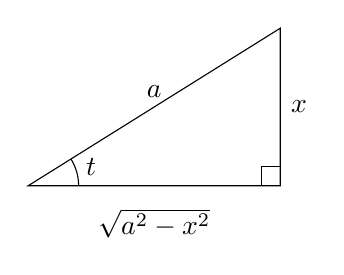
\begin{tikzpicture}[scale=0.8]

                    % 定义点
                    \coordinate (O) at (0,0);
                    \coordinate (A) at (4,0);
                    \coordinate (B) at (4,2.5);

                    % 画三角形
                    \draw (O) -- (A) -- (B) -- cycle;

                    % 直角符号
                    \draw (3.7,0) -- (3.7,0.3) -- (4,0.3);

                    % 标注边
                    \node at (2, -0.6) {$\gmath{\sqrt{a^2 - x^2}}$};
                    \node at (4.3, 1.25) {$x$};
                    \node at (2, 1.5) {$a$};

                    % 标注角 t
                    \draw (0.8,0) arc (0:32:0.8);
                    \node at (1,0.3) {$t$};
                \end{tikzpicture}
            \end{center}
            \item $\sqrt {a^2 + x^2} \Rightarrow$ 令$x = a\tan t, |t| < \displaystyle\frac{\pi}{2}$
            \begin{center}
                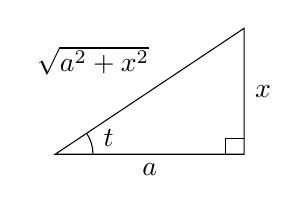
\begin{tikzpicture}[scale=0.8]

                    % 定义点
                    \coordinate (O) at (0,0);
                    \coordinate (A) at (3,0);
                    \coordinate (B) at (3,2);

                    % 画三角形
                    \draw (O) -- (A) -- (B) -- cycle;

                    % 直角符号
                    \draw (2.7,0) -- (2.7,0.25) -- (3,0.25);

                    % 标注边
                    \node at (1.5,-0.25) {$a$};
                    \node at (3.3,1) {$x$};
                    \node[above] at (0.6,1.1) {$\gmath{\sqrt{a^2 + x^2}}$};

                    % 标注角 t
                    \draw (0.6,0) arc (0:34:0.6);
                    \node at (0.85,0.25) {$t$};

                \end{tikzpicture}
            \end{center}
            \item $\sqrt {x^2 - a^2} \Rightarrow$ 令$x = a\sec t$
            \[
                \begin{cases}
                    x > 0 \;\Longrightarrow\; 0 < t < \dfrac{\pi}{2}, \\[6pt]
                    x < 0 \;\Longrightarrow\; \dfrac{\pi}{2} < t < \pi.
                \end{cases}
            \]
        \end{itemize}
        \item 恒等变形后作三角函数代换：当被积函数含有根式$\sqrt {ax^2 + bx + c}$时，可先化为$\sqrt {\varphi^2(x) + k^2}$、$\sqrt {\varphi^2(x) - k^2}$或$\sqrt {k^2 - \varphi^2(x)}$，再作三角函数代换
        \item ${\color{red}{\bigstar}}$根式代换：当被积函数含有根式$\sqrt[n]{ax + b}, \sqrt {\displaystyle\frac{ax + b}{cx + d}}, \sqrt {ae^{bx} + c}$时，一般令根式$\sqrt {*} = t$。对既含有$\sqrt[n]{ax + b}$，也含有$\sqrt[m]{ax + b}$的函数，一般取$m, n$的最小公倍数$l$，令$\sqrt[l]{ax + b} = t$
        \item 倒代换：当被积函数{\color{red}{分母}}的幂次比{\color{red}{分子}}高两次及两次以上时，作倒代换，令$x = \dfrac{1}{t}$
        \item 复杂函数的直接代换：当被积函数中含有$a^x, e^x, \ln x, \arcsin x, \arctan x$等时，可考虑直接令复杂函数等于$t$
    \end{enumerate}

    \subsubsection{分部积分法}

    \begin{enumerate}
        \item $\int u\,\mathrm{d}v = uv - \int v\,\mathrm{d}u$(反对幂指三)
        \item 设函数$u = u(x)$与$v = v(x)$具有直到第$n+1$阶的连续导数，并根据分部积分公式$\int u\,\mathrm{d}v = uv - \int v\,\mathrm{d}u$则有
        \[
            \int {\color{red}{uv^{(n+1)}}}\,\mathrm{d}x = uv^{(n)} - u'v^{(n-1)} + u''v^{(n-2)}- \cdots + (-1)^{n}u^{(n)}v + (-1)^{n+1}\int u^{(n+1)}v\,\mathrm{d}x
        \]

        \begin{center}
            \begin{aligned}
                \int uv^{(4)}\,\mathrm{d}x
                &= \begin{tabular}{c|c|c|c|c|c}
                       \hline
                       $u$\text{各阶导数}       & $u$     & $u'$    & $u''$ & $u^{(3)}$ & $u^{(4)}$ \\
                       \hline
                       $v^{(4)}$\text{各阶导数} & v^{(4)} & v^{(3)} & $v''$ & $v'$      & $v$       \\
                       \hline
                \end{tabular} \\
                &= uv^{(3)} - u'v'' + u''v' - u^{(3)}v + \int u^{(4)}v\,\mathrm{d}x
            \end{aligned}
        \end{center}

        计算方法：以$u$作起点左上、右下错位相乘，各项符号 $+,-,$ 相间，最后一项为$\int u^{(4)}v\,\mathrm{d}x$
        \item 分部积分法可能的结果
        \begin{itemize}
            \item 方程: $I = \square - I$
            \item 抵消: $I = \square - I_1 + I_1$
            \item 递推式: $I_n = F(I_{n-1}, I_{n-2})$
        \end{itemize}

    \end{enumerate}

    \subsubsection{有理函数的积分}

    \begin{enumerate}
        \item 定义：形如$\dint \displaystyle\frac{P_n(x)}{Q_m(x)}\,\mathrm{d}x(n < m)$的积分称为\textbf{有理函数的积分}，其中$P_n(x), Q_m(x)$分别是$x$的$n$次多项式和$m$次多项式
        \item 思想：若$Q_m(x)$在实数域内可因式分解，则因式分解后再把$\displaystyle\frac{P_n(x)}{Q_m(x)}$拆成若干项最简有理分式之和。有理式$=$\textbf{最简有理分式之和}，其中最简有理式分为
        \begin{circlenum}
            \item $\displaystyle\frac{A}{ax + b}$
            \item $\displaystyle\frac{A_k}{(ax + b)^k}, k=2,3,\cdots$
            \item $\displaystyle\frac{Ax + B}{px^2 + qx + r}$
            \item $\displaystyle\frac{A_{k}x + B_k}{(px^2 + qx + r)^k}, k=2,3,\cdots$
        \end{circlenum}
        \item 方法（如何拆）
        \begin{circlenum}
            \item $Q_m(x)$的一次单因式产生一项$\displaystyle\frac{A}{ax + b}$
            \begin{analysisbox}[Example]
                \[
                    \int \frac{1}{x + 1}\,\mathrm{d}x = \ln |x+1| + C
                \]
            \end{analysisbox}
            \item $Q_m(x)$的$k$重一次因式$(ax + b)^k$产生$k$项，分别为$\displaystyle\frac{A_1}{ax + b}, \displaystyle\frac{A_2}{(ax + b)^2}, \cdots, \displaystyle\frac{A_k}{(ax + b)^k}, k = 2,3,\cdots$
            \begin{analysisbox}[Example]
                \[
                    \int \frac{2}{(2x-1)^2}\,\mathrm{d}x = \int \frac{1}{(2x-1)^2}\,\mathrm{d}(2x-1) = -\frac{1}{2x-1} + C
                \]
            \end{analysisbox}
            \item $Q_m(x)$的二次单因式$px^2 + qx + r$产生一项$\displaystyle\frac{Ax + B}{px^2 + qx + r}$。须$\Delta = q^2 - 4pr < 0$，拆出单因式后，使用$\dint \dfrac{1}{a^2 + x^2}\,\mathrm{d}x = \displaystyle\frac{1}{a}\arctan \displaystyle\frac{x}{a} + C, a > 0$
            \begin{analysisbox}[Example]
                \[
                    \int \frac{x-1}{x^2 + 1}\,\mathrm{d}x = \int \frac{1}{2}\frac{2x}{x^2 + 1}\,\mathrm{d}x - \int \frac{1}{x^2 + 1}\,\mathrm{d}x = \frac{1}{2}\ln (x^2 + 1) - \arctan x + C
                \]
            \end{analysisbox}
            \item $Q_m(x)$的$k$重二次因式$(px^2 + qx + r)^k$产生$k$项，分别为$\displaystyle\frac{A_{1}x + B_1}{px^2 + qx + r}$，$\displaystyle\frac{A_{2}x + B_2}{(px^2 + qx + r)^2}$，$\cdots, \displaystyle\frac{A_{k}x + B_k}{(px^2 + qx + r)^k}$
            \begin{analysisbox}[Example]
                求
                \[
                    I_2 = \int \frac{\mathrm{d}x}{(1+x^2)^2}.
                \]

                \textbf{思路：}
                若分母为 $1+x^2$，则原函数为 $\arctan x$，
                因此考虑将 $(1+x^2)^2$ 降阶处理。

                \textbf{解：}
                设
                \[
                    I_1 = \int \frac{1}{1+x^2}\,\mathrm{d}x = \arctan x.
                \]

                利用分部积分法，
                \[
                    I_1
                    = \int \frac{1}{1+x^2}\,\mathrm{d}x
                    = \frac{x}{1+x^2}
                    + \int x \cdot \frac{2x}{(1+x^2)^2}\,\mathrm{d}x.
                \]

                整理被积式：
                \[
                    \begin{aligned}
                        I_1
                        &= \frac{x}{1+x^2}
                        + 2 \int \frac{x^2}{(1+x^2)^2}\,\mathrm{d}x \\
                        &= \frac{x}{1+x^2}
                        + 2 \int \frac{(1+x^2)-1}{(1+x^2)^2}\,\mathrm{d}x \\
                        &= \frac{x}{1+x^2}
                        + 2 \int \frac{1}{1+x^2}\,\mathrm{d}x
                        - 2 \int \frac{1}{(1+x^2)^2}\,\mathrm{d}x.
                    \end{aligned}
                \]

                即
                \[
                    I_1
                    = \frac{x}{1+x^2}
                    + 2I_1
                    - 2I_2.
                \]

                解得
                \[
                    I_2
                    =
                    \frac{x}{2(1+x^2)}
                    +
                    \frac{1}{2}\arctan x
                    + C.
                \]
            \end{analysisbox}
            \item \begin{analysisbox}[Example]
                      \[
                          \frac{4x^2 - 6x - 1}{(x+1)(2x-1)^2}
                          =
                          \frac{A}{x+1}
                          +
                          \frac{B}{2x-1}
                          +
                          \frac{C}{(2x-1)^2}
                      \]

                      解恒等式：
                      \[
                          A(2x-1)^2
                          +
                          B(x+1)(2x-1)
                          +
                          C(x+1)
                          =
                          4x^2 - 6x - 1
                      \]

                      在恒等式中，对变量 $x$ 取任意值，等式两边应恒相等，
                      因此可代入特殊值求系数。

                      令
                      \[
                          x = -1,
                          \quad
                          x = \frac{1}{2},
                          \quad
                          x = 0
                      \]
                      即可求得 $A, B, C$
            \end{analysisbox}
        \end{circlenum}
    \end{enumerate}

    \subsection{定积分的计算}

    \subsubsection{牛顿-莱布尼茨公式}
    设函数$F(x)$是连续函数$f(x)$在$[a, b]$上的一个原函数，则
    \[
        \int_a^b f(x)\,\mathrm{d}x = F(x)\Big|_{a}^{b} = F(b) - F(a)
    \]

    \subsubsection{牛顿–莱布尼茨公式的推广}

    设 $f(x)$ 在 $[a,b]$ 上分段存在原函数。
    若在 $[a,c)$ 上存在原函数 $F_1(x)$，
    在 $(c,b]$ 上存在原函数 $F_2(x)$，
    则

    \[
        \int_a^b f(x)\,\mathrm{d}x
        =
        \int_a^c f(x)\,\mathrm{d}x
        +
        \int_c^b f(x)\,\mathrm{d}x.
    \]

    若极限存在，则

    \[
        \int_a^b f(x)\,\mathrm{d}x
        =
        \lim_{x \to c^-} F_1(x) - F_1(a)
        +
        F_2(b) - \lim_{x \to c^+} F_2(x).
    \]

    \medskip

    \textbf{收敛性判定：}

    \begin{itemize}
        \item 若 $\displaystyle \lim_{x \to c^-} F_1(x)$ 与
        $\displaystyle \lim_{x \to c^+} F_2(x)$ 均存在，
        则 $\displaystyle \int_a^b f(x)\,\mathrm{d}x$ 收敛；

        \item 若上述两个极限中至少有一个不存在，
        则 $\displaystyle \int_a^b f(x)\,\mathrm{d}x$ 发散。
    \end{itemize}

    \subsubsection{定积分的换元积分法}

    设$f(x)$在$[a, b]$上连续，函数$x = \varphi(t)$满足\ding{172}$\varphi(\alpha) = a, \varphi(\beta) = b$; \ding{173}$x = \varphi(t)$在$[\alpha, \beta]$（或$[\beta, \alpha]$）上有连续的导数，且其值域为$R_\varphi = [a, b]$，则有
    \[
        \int_a^b f(x)\,\mathrm{d}x = \int_{\alpha}^{\beta} f[\varphi(t)]\varphi'(t)\,\mathrm{d}t
    \]

    \textbf{\color{red}{换元要三换}}
    \begin{circlenum}
        \item 被积函数要换: $f(x) \rightarrow f[\varphi(x)]$
        \item 积分变量要换: $\mathrm{d}x \rightarrow \varphi'(t)\,\mathrm{d}t$
        \item 上下限要换: $\int_{a}^b \rightarrow \int_{\alpha}^{\beta}$
    \end{circlenum}

    \subsubsection{定积分的分部积分法}

    \[
        \int_a^b u(x)v'(x)\,\mathrm{d}x = u(x)v(x)\Big|_a^b - \int_a^b v(x)u'(x)\,\mathrm{d}x
    \]
    这里要求$u'(x), v'(x)$在$[a, b]$上连续

    \subsubsection{结论}

    \begin{enumerate}
        \item 设$f(x)$为连续的偶函数，则$\dint_{-a}^{a} f(x)\,\mathrm{d}x = 2\dint_{0}^{a} f(x)\,\mathrm{d}x$
        \item 设$f(x)$为连续的奇函数，则$\dint_{-a}^{a} f(x)\,\mathrm{d}x = 0$
        \item 设$f(x)$是以$T$为周期的连续函数，则$\dint_{a}^{a + T} f(x)\,\mathrm{d}x = \dint_{0}^{T} f(x)\,\mathrm{d}x$
        \item 区间再现公式：设$f(x)$为连续函数，则$\dint_{a}^{b} f(x)\,\mathrm{d}x = \dint_{a}^{b} f(a + b - x)\,\mathrm{d}x$
        \begin{enumerate}
            \item 若$f(x)$复杂，$f(x) + f(a + b - x)$简单，则考虑
            \[
                \int_a^b f(x)\,\mathrm{d}x = \int_a^b \frac{f(x) + f(a + b - x)}{2}\,\mathrm{d}x
            \]
            \item \classic{经典}
            \[
                \begin{aligned}
                    \int_0^{\frac{\pi}{4}} \ln(1+\tan x)\,\mathrm{d}x
                    &\xlongequal{x=\frac{\pi}{4}-t}
                    \ln\!\left[1+\tan\!\left(\frac{\pi}{4}-x\right)\right]
                    \,\mathrm{d}x \\[6pt]
                    &= \int_0^{\frac{\pi}{4}}
                    \ln\!\left(\frac{2}{1+\tan x}\right)
                    \,\mathrm{d}x \\[6pt]
                    &= \int_0^{\frac{\pi}{4}}
                    \frac{
                        \ln\!\left(\frac{2}{1+\tan x}\right)
                        +
                        \ln(1+\tan x)
                    }{2}
                    \,\mathrm{d}x \\[8pt]
                    &= \frac{\pi}{8}\ln 2
                \end{aligned}
            \]
            \item $\dint_0^{\pi} xf(\sin x)\,\mathrm{d}x \xlongequal{x=\pi-t} \dfrac{\pi}{2}\dint_0^{\pi} f(\sin x)\,\mathrm{d}x$
        \end{enumerate}
        \item 华里士公式(点火公式)
        \begin{itemize}
            \item \[
                      \int_{0}^{\frac{\pi}{2}} \sin^{n} x \,\mathrm{d}x
                      =
                      \int_{0}^{\frac{\pi}{2}} \cos^{n} x \,\mathrm{d}x
                      =
                      \begin{cases}
                          \displaystyle
                          \frac{n-1}{n}
                          \cdot
                          \frac{n-3}{n-2}
                          \cdot
                          \cdots
                          \cdot
                          \frac{2}{3}
                          \cdot
                          1,
                          & n \text{为大于 1 的奇数}, \\[1.2em]

                          \displaystyle
                          \frac{n-1}{n}
                          \cdot
                          \frac{n-3}{n-2}
                          \cdot
                          \cdots
                          \cdot
                          \frac{1}{2}
                          \cdot
                          \frac{\pi}{2},
                          & n \text{为正偶数}.
                      \end{cases}
            \]

            \item
            \[
                \int_{0}^{\pi} \sin^{n} x \,\mathrm{d}x
                =
                \begin{cases}
                    \displaystyle
                    2
                    \cdot
                    \frac{n-1}{n}
                    \cdot
                    \frac{n-3}{n-2}
                    \cdot
                    \cdots
                    \cdot
                    \frac{2}{3}
                    \cdot
                    1,
                    & n \text{为大于 1 的奇数}, \\[1.2em]

                    \displaystyle
                    2
                    \cdot
                    \frac{n-1}{n}
                    \cdot
                    \frac{n-3}{n-2}
                    \cdot
                    \cdots
                    \cdot
                    \frac{1}{2}
                    \cdot
                    \frac{\pi}{2},
                    & n \text{为正偶数}.
                \end{cases}
            \]

            \[
                \int_{0}^{\pi} \cos^{n} x \,\mathrm{d}x
                =
                \begin{cases}
                    0,
                    & n \text{为正奇数}, \\[0.8em]

                    \displaystyle
                    2
                    \cdot
                    \frac{n-1}{n}
                    \cdot
                    \frac{n-3}{n-2}
                    \cdot
                    \cdots
                    \cdot
                    \frac{1}{2}
                    \cdot
                    \frac{\pi}{2},
                    & n \text{为正偶数}.
                \end{cases}
            \]

            \item
            \[
                \int_{0}^{2\pi} \sin^{n} x \,\mathrm{d}x
                =
                \int_{0}^{2\pi} \cos^{n} x \,\mathrm{d}x
                =
                \begin{cases}
                    0,
                    & n \text{为正奇数}, \\[0.8em]

                    \displaystyle
                    4
                    \cdot
                    \frac{n-1}{n}
                    \cdot
                    \frac{n-3}{n-2}
                    \cdot
                    \cdots
                    \cdot
                    \frac{1}{2}
                    \cdot
                    \frac{\pi}{2},
                    & n \text{为正偶数}.
                \end{cases}
            \]
        \end{itemize}
    \end{enumerate}

    \subsection{变限积分的计算}

    \subsubsection{求导公式}

    设$F(x) = \dint_{\varphi_1(x)}^{\varphi_2(x)} {\color{red}{f(t)}}\,\mathrm{d}t$，其中$f(x)$在$[a, b]$上连续，可导函数$\varphi_1(x)$和$\varphi_2(x)$的值域在$[a, b]$上，则在函数$\varphi_1(x)$和$\varphi_2(x)$的公共定义域上，有
    \[
        F'(x) = \frac{\mathrm{d}}{\mathrm{d}x}\left[\int_{\varphi_1(x)}^{\varphi_2(x)} f(t)\,\mathrm{d}t\right] = f[\varphi_2(x)]\varphi_2'(x) - f[\varphi_1(x)]\varphi_1'(x)
    \]

    上面公式中的$x$为\textbf{求导变量}，$t$为\textbf{积分变量}。当被积函数中只含\textbf{积分变量}$t$时，才能使用求导公式，若被积函数中有\textbf{求导变量}$x$，则必须通过恒等变形（比如变量代换等）将其移出被积函数，才能使用变限积分求导公式

    \subsubsection{重要结论}

    只需要被积函数可积，即可有变限积分的相关性质，只有被积函数连续时，才能谈原函数的相关性质

    \begin{enumerate}

        \item ${\color{red}{\bigstar}}$\; $f(x)$ 为可积（\textbf{有可能有跳跃间断点、可去间断点}）的奇函数 $\Rightarrow \dint_{a}^{x} f(t)\,\mathrm{d}t,\ \forall a$ 为偶函数

        \item 若 $f(x)$ 为连续的奇函数，则 $\dint_{a}^{x} f(t)\,\mathrm{d}t + C$ 也是偶函数，故 $f(x)$ 的全体原函数均为偶函数

        \item ${\color{red}{\bigstar}}$\; $f(x)$ 为可积的偶函数 $\Rightarrow$
        \[
            \begin{cases}
                \dint_{0}^{x} f(t)\,\mathrm{d}t \text{ 为奇函数}, \\[6pt]
                \dint_{a}^{x} f(t)\,\mathrm{d}t \ (a \neq 0)
                \begin{cases}
                    \text{若 } \dint_{a}^{x} f(t)\,\mathrm{d}t
                    =
                    \dint_{0}^{x} f(t)\,\mathrm{d}t, \text{ 为奇函数}, \\[6pt]
                    \text{若 } \dint_{a}^{x} f(t)\,\mathrm{d}t
                    \neq
                    \dint_{0}^{x} f(t)\,\mathrm{d}t, \text{ 为非奇非偶函数}.
                \end{cases}
            \end{cases}
        \]
        \begin{analysisbox}[Example]

            判断函数
            \[
                f(x)=\int_0^{\sin x} \cos t^2\,\mathrm{d}t
            \]
            的奇偶性。

            令
            \[
                h(x)=\int_0^{x} \cos t^2\,\mathrm{d}t,
            \]
            则
            \[
                f(x)=h(\sin x)=h\bigl(g(x)\bigr),
                \quad g(x)=\sin x.
            \]

            由于 $\cos t^2$ 为偶函数，
            故 $h(x)$ 为奇函数；

            又 $g(x)=\sin x$ 为奇函数，

            因此
            \[
                f(x)=h(g(x))
            \]
            为奇函数。

        \end{analysisbox}

        \item 若 $f(x)$ 为连续的偶函数，则 $f(x)$ 的全体原函数中，只有 $\dint_{0}^{x} f(t)\,\mathrm{d}t$ 是奇函数

        \item $f(x)$ 是可积且以 $T$ 为周期的周期函数，则 $\dint_{0}^{x} f(t)\,\mathrm{d}t$ 是以 $T$ 为周期的周期函数 $\Leftrightarrow \dint_{0}^{T} f(x)\,\mathrm{d}x = 0 \Leftrightarrow \dint_{a}^{x} f(t)\,\mathrm{d}t = \dint_{a}^{0} f(t)\,\mathrm{d}t + \dint_{0}^{x} f(t)\,\mathrm{d}t$ 亦是以 $T$ 为周期的周期函数 $(a \neq 0)$
        \item 若被积函数中含有绝对值，可以通过拆分区间来消去绝对值

    \end{enumerate}

    \subsection{反常积分的计算}

    \begin{enumerate}
        \item 在计算反常积分时，注意识别奇点（端点、{\color{red}{内部}}）(瑕点，$\pm \infty$)
        \item 反常积分在收敛的情况下，通过换元可能实现反常积分与定积分的相互转化
    \end{enumerate}

    \subsection{基础概念}

    \begin{enumerate}
        \item \textbf{$\Gamma$函数}

        \textbf{定义：}
        \[
            \begin{aligned}
                \Gamma(\alpha)
                &= \int_{0}^{+\infty} x^{\alpha-1} e^{-x}\,\mathrm{d}x
                &\xlongequal{\;x=t^2\;} \, 2\int_{0}^{+\infty} t^{2\alpha-1} e^{-t^2}\,\mathrm{d}t (\alpha, t > 0).
            \end{aligned}
        \]

        \textbf{递推公式：}

        \[
            \begin{aligned}
                \Gamma(\alpha+1)
                &= \int_{0}^{+\infty} x^{\alpha} e^{-x}\,\mathrm{d}x \\
                &= -\int_{0}^{+\infty} x^{\alpha}\,\mathrm{d}(e^{-x}) \\
                &= -x^{\alpha} e^{-x}\Big|_{0}^{+\infty}
                + \int_{0}^{+\infty} e^{-x}\alpha x^{\alpha-1}\,\mathrm{d}x \\
                &= \alpha \Gamma(\alpha).
            \end{aligned}
        \]

        \textbf{特殊值：}

        \[
            \Gamma(1)=1,
            \qquad
            \Gamma\!\left(\frac{1}{2}\right)=\sqrt{\pi}.
        \]

        因此
        \begin{gather*}
            \Gamma(n+1)=n! \\
            \Gamma\!\left(\frac{5}{2}\right)
            = \frac{3}{2}\cdot\frac{1}{2}\cdot\Gamma\!\left(\frac{1}{2}\right)
            = \frac34\sqrt{\pi}.\\
        \end{gather*}
    \end{enumerate}

    \subsection{运算}

    \begin{enumerate}

        \item
        \[
            \begin{aligned}
                \int \frac{1}{1+e^x}\,\mathrm{d}x
                &=
                \int \left(1 - \frac{e^x}{1+e^x}\right)\,\mathrm{d}x
            \end{aligned}
        \]

        \item
        \[
            \begin{aligned}
                \int_0^1 \arcsin \sqrt{1 - x^2}\,\mathrm{d}x
                &=
                x \arcsin \sqrt {1 - x^2}\Big|_0^1 - \int_0^1 x\,\mathrm{d}(\arcsin \sqrt{1 - x^2}) \\[6pt]
                &=
                \int_0^1 \frac{x}{\sqrt{1 - x^2}}\,\mathrm{d}x  \\[6pt]
                &=
                -\sqrt{1 - x^2}\Big|_0^1  \\[6pt]
                &=
                1
            \end{aligned}
        \]
        \item
        \[
            \begin{aligned}
                \int \cos^{3} t \,\mathrm{d}t
                &= \int (1 - \sin^2 t)\cos t \,\mathrm{d}t \\[6pt]
                &= \int (1-\sin^2 t)\,\mathrm{d}(\sin t) \\[6pt]
                &= \sin t - \frac{\sin^3 t}{3} + C.
            \end{aligned}
        \]

    \end{enumerate}

    \subsection{公式}

    \begin{enumerate}
        \item
        \[
            \begin{aligned}
                \int e^{ax} \sin bx \,\mathrm{d}x
                &=
                \frac{
                    \begin{vmatrix}
                        (e^{ax})' & (\sin bx)' \\
                        e^{ax} & \sin bx
                    \end{vmatrix}
                }{a^2 + b^2}
                + C  \\[6pt]
                &=
                \frac{a e^{ax} \sin bx - b e^{ax} \cos bx}{a^2 + b^2}
                + C
            \end{aligned}
        \]

        \item
        \[
            \begin{aligned}
                \int e^{ax} \cos bx \,\mathrm{d}x
                &=
                \frac{
                    \begin{vmatrix}
                        (e^{ax})' & (\cos bx)' \\
                        e^{ax} & \cos bx
                    \end{vmatrix}
                }{a^2 + b^2}
                + C \\[6pt]
                &=
                \frac{a e^{ax} \cos bx + b e^{ax} \sin bx}{a^2 + b^2}
                + C
            \end{aligned}
        \]
        \item $I_n = \dint_0^{+\infty} x^ne^{-x}\,\mathrm{d}x = n!(n\text{为非负整数})$
        \item $\tan (\dfrac{\pi}{4} - \alpha) = \displaystyle\frac{1 - \tan \alpha}{1 + \tan \alpha}$
        \item
        \[
            \int \sqrt{1+x^2}\,\mathrm{d}x
            =
            \frac{x\sqrt{1+x^2}}{2}
            +
            \frac{1}{2}\ln\!\left(x+\sqrt{1+x^2}\right)
            + C
        \]

    \end{enumerate}

    \subsection{方法总结}

    \begin{enumerate}
        \item 若不是常用的凑微分公式，则可对被积函数的复杂部分$g(x)$求导，若$g'(x) = f(x)$，即$d[g(x)] = f(x)dx$，则$\dint f(x)g(x)\,\mathrm{d}x = \int g(x)\,\mathrm{d}[g(x)]$，凑微分成功
        \item $\dint \triangle\,\mathrm{d}x$一般不好求，可将其转化成$\dint \nabla\,\mathrm{d}x$
        \item 形如$R(\sin x, \cos x)$的有理式称为三角函数有理式
        \begin{enumerate}
            \item 令$t = \tan \displaystyle\frac{x}{2},\, \sin x = \displaystyle\frac{2t}{1 + t^2},\, \cos x = \displaystyle\frac{1-t^2}{1+t^2}$
            \item 凑微分
            \begin{itemize}
                \item 若$R(\sin x, \cos x) = -R(-\sin x, \cos x)$，令$\cos x = t$。$\sin$是奇数次方，\emph{e.g.} $\displaystyle\frac{\sin^5 x}{\cos^4 x} = -\displaystyle\frac{-\sin^5 x}{\cos^4 x}$
                \item 若$R(\sin x, \cos x) = -R(\sin x, -\cos x)$，令$\sin x = t$。$\cos$是奇数次方
                \item 若$R(\sin x, \cos x) = R(-\sin x, -\cos x)$，令$\tan x = t$
            \end{itemize}
        \end{enumerate}
        \item 定积分计算时考虑{\color{customgreen}{奇偶性}}和{\color{customgreen}{周期性}}，做{\color{customgreen}{平移代换}}。\emph{e.g.}\,$\dint_0^1 \Rightarrow? \dint_{-\frac{1}{2}}^{\frac{1}{2}}$
        \item $\dfrac{1}{1+\sin x}$分母有理化（恒等变形）
    \end{enumerate}

\end{document}
